\documentclass{report}

\usepackage{tikz}
\usepackage{float}
\usepackage{lscape}
\usepackage{multicol}
\usepackage{datetime}
\usepackage{booktabs}
\usepackage{pgfplots}
\usepackage[top=1cm,left=1cm,right=1cm,bottom=1cm]{geometry}

% \title{Electromagnetic Labs}
% \author{Shawal Mbalire \\21/U/0851 \\BELE}
\pgfplotsset{compat=1.18}
\usetikzlibrary{shapes, arrows, positioning}

\begin{document}
    \begin{titlepage}
        \begin{center}
            % \maketitle
        {\huge\bfseries A report on an Experiment of comparison between matched and mismatched loads\\}
        % ----------------------------------------------------------------
        \vspace{1.5cm}
        {\Large\bfseries Shawal Mbalire}\\[5pt]
        \bfseries mbalireshawal@gmail.com\\[14pt]
        % ----------------------------------------------------------------
        \vspace{1cm}
        
        \begin{table}[ht]
            \centering
            \begin{tabular}{lll}
            \toprule
            NAME & REG NUMBER \\
            \midrule
            AMUTUHIRE JUDITH & 22/U/5773 \\
            AINE MUGABE HILLARY & 22/U/5683 \\
            ACHOLA LOY ABOR & 22/U/5637 \\
            SSEKAJJA HENRY & 22/U/6907 \\
            ANKWASA DERRICK & 22/U/5780 \\
            KYEYUNE JORDIE & 20/U/0449 \\
            ARANSIOLA OYINDAMOLA SERENA & 21/X/20031/ps \\
            BUJINGO MATTHEW & 22/U/5895 \\
            MBALIRE SHAWAL & 21/U/0851 \\
            AGABA TIMOTHY TRAVIS & 22/U/23062 \\
            \bottomrule
            \end{tabular}
            \caption{Group 1 Members}
            \label{tab:student_info}
        \end{table}

        \vfill
        % ----------------------------------------------------------------
        \includegraphics[width=0.7\textwidth]{makLogo.png}\\
        \vspace{0.4cm}
        {\Large\bfseries College of Engineering Design Art and Technology}\\ 
        \vspace{0.4cm}
        {\Large\bfseries Department of Electrical and Computer Engineering}\\
        \vspace{0.4cm}
        {\Large\bfseries Bachelor of Science in Electrical Engineering}\\
        \vfill
        {\today}
        \end{center}
    \end{titlepage}
    % \maketitle

    \tableofcontents
    \chapter{Introduction}
    \section{Objectives}
    The objective of the practical is to understand the differences between a matched load and a mismatched load and different grades of mismatched loads. We will compare the results and we will recognise the different types of loads.

    \section{Equipment}
    \begin{enumerate}
        \item Interface
        \item Gunn oscillator
        \item Waveguide slotted linewidth
        \item 6dB fixed attenuator
        \item Termination load
        \item Short circuit
        \item Horizontal variable attenuator
    \end{enumerate}
    \chapter{Procedure}
    The experiment was carried out following the procedure as listed below
    \begin{enumerate}
    \item First of all, the first circuit ("Mismatched Load 1") that consists of a gunn oscillator,  a horizontal variable attenuator, a slotted line and a short circuit was assembled.  
    \begin{figure}[H]
    
\begin{tikzpicture}[node distance=2cm]
        % Draw the blocks
        \node (gunn)    [draw, rectangle, minimum width=2cm, minimum height=1cm] {Gunn Oscillator};
        \node (hva)     [draw, rectangle, minimum width=2cm, minimum height=1cm,  right=of gunn] {Horizontal V Attenuator};
        \node (slotted) [draw, rectangle, minimum width=2cm, minimum height=1cm,  right=of hva] {Slotted Line};
        \node (short)   [draw, rectangle, minimum width=2cm, minimum height=1cm, right=of slotted] {Short Circuit};
      
        % Draw the connecting line
        \draw [->] (gunn) -- (hva);
        \draw [->] (hva) -- (slotted);
        \draw [->] (slotted) -- (short);
      
        % Add some arrows to the connections
        \draw [->] (gunn) -- node [above] {} (hva);
        \draw [->] (hva) -- node [above] {} (slotted);
        \draw [->] (slotted) -- node [above] {} (short);
    \end{tikzpicture}
    \caption{Microwave crcuit with mismatched load 1}
    \end{figure}
    \item The gunn oscilator element is connected to the gunn oscilatorpower supply connector. The power meter is connected to the power meter "RF Input" connector.
    \item The micrometer of the horizontal variable attenuator is set to the 2mm position
    \item The diode dector of the slotted line is set to the 0 mm position
    \item After verifying that the circuit breaker is on, the unit is switched on.
    \item The detector in the ssloted line is moved slowly until maximum power is reached.
    \item The position of the micrometer is moved slowly until the maximum power signal detected is between 0.800mW and 0.850mW. With this attenuation, the diode detector is prevented from saturation.
    \item With the diode detector mount in 0mm, the diode mount of the slottedline is increased slowly while recording the value of SWR meter display every millimeter until the 40 mm position
    \item The unit is turned off
    \item The reflected power is calculated with the equation included below 
    \[SWR = \frac{V_{max}}{V_{min}}\]\[ Power_{reflected} = \left( \frac{SWR-1}{SWR+1} \right)^2 \] . In real systems, the reflected power is the powersignal that goes back to the generator and it should be minimised in order to avoid the gneraator to be damaged.
    \item Now the second circuit ("Mismatched Load 2") is assembled that consists a gunn oscillator, horizontal variable attenuator, 6dB fixed attenuator and short circuit as shown in the figure below.
    \begin{figure}[H]
    
\begin{tikzpicture}[node distance=1cm]
        % Draw the blocks
        \node (gunn)    [draw, rectangle, minimum width=2cm, minimum height=1cm] {Gunn Oscillator};
        \node (hva)     [draw, rectangle, minimum width=2cm, minimum height=1cm,  right=of gunn] {Horizontal V Attenuator};
        \node (slotted) [draw, rectangle, minimum width=2cm, minimum height=1cm,  right=of hva] {Slotted Line};
        \node (six)   [draw, rectangle, minimum width=2cm, minimum height=1cm, right=of slotted] {6dB fixed attenuator};
        \node (short)   [draw, rectangle, minimum width=2cm, minimum height=1cm, right=of six] {Short Circuit};
      
        % Draw the connecting line
        \draw [->] (gunn) -- (hva);
        \draw [->] (hva) -- (slotted);
        \draw [->] (slotted) -- (six);
        \draw [->] (six) -- (short);
      
        % Add some arrows to the connections
        \draw [->] (gunn) -- node [above] {} (hva);
        \draw [->] (hva) -- node [above] {} (slotted);
        \draw [->] (slotted) -- node [above] {} (six);
        \draw [->] (six) -- node [above] {} (short);
    \end{tikzpicture}
    \caption{Microwave crcuit with mismatched load 2}
    \end{figure}
    \item Steps 2 through 10 are repeated and reflected power is calculated.
    \item Finally the third circuit ("Matched Load") is assembled that consists a gunn oscillator, horizontal variable attenuator, and termination load as shown in the figure below.
    \begin{figure}[H]
    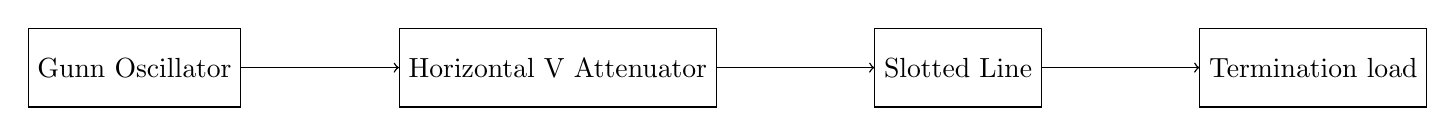
\begin{tikzpicture}[node distance=2cm]
        % Draw the blocks
        \node (gunn)    [draw, rectangle, minimum width=2cm, minimum height=1cm] {Gunn Oscillator};
        \node (hva)     [draw, rectangle, minimum width=2cm, minimum height=1cm,  right=of gunn] {Horizontal V Attenuator};
        \node (slotted) [draw, rectangle, minimum width=2cm, minimum height=1cm,  right=of hva] {Slotted Line};
        \node (short)   [draw, rectangle, minimum width=2cm, minimum height=1cm, right=of slotted] {Termination load};
      
        % Draw the connecting line
        \draw [->] (gunn) -- (hva);
        \draw [->] (hva) -- (slotted);
        \draw [->] (slotted) -- (short);
      
        % Add some arrows to the connections
        \draw [->] (gunn) -- node [above] {} (hva);
        \draw [->] (hva) -- node [above] {} (slotted);
        \draw [->] (slotted) -- node [above] {} (short);
    \end{tikzpicture}
    \caption{Microwave crcuit with matched load}
    \end{figure}
    \item Steps 2 through 10 are repeated and reflected power is calculated.
    \item The results are compared and the load with the worst SWR is identified
    \item Using a smith chart, the SWR and reflection coefficient of all loads are calculated.
    \end{enumerate}
    \[ coefficient_{reflection} = \frac{SWR-1}{SWR+1} \] 

    \chapter{Theory}
    \chapter{Results}
    
    \section{Mismatched Load 1}
    \begin{multicols}{2}
    \begin{table}[H]
        \centering
        \begin{tabular}{cc}
        \hline
        Length(mm) & Column 2 \\
        \hline
        0.00 & 0.113 \\
        0.01 & 0.144 \\
        0.02 & 0.187 \\
        0.03 & 0.231 \\
        0.04 & 0.279 \\
        0.05 & 0.312 \\
        0.06 & 0.349 \\
        0.07 & 0.416 \\
        0.08 & 0.471 \\
        0.09 & 0.516 \\
        0.10 & 0.574 \\
        0.11 & 0.631 \\
        0.12 & 0.684 \\
        0.13 & 0.721 \\
        0.14 & 0.746 \\
        0.15 & 0.736 \\
        0.16 & 0.601 \\
        0.17 & 0.195 \\
        0.18 & 0.119 \\
        0.19 & 0.139 \\
        0.20 & 0.176 \\
        0.21 & 0.207 \\
        0.22 & 0.250 \\
        0.23 & 0.287 \\
        0.24 & 0.326 \\
        0.25 & 0.380 \\
        0.26 & 0.434 \\
        0.27 & 0.512 \\
        0.28 & 0.567 \\
        0.29 & 0.620 \\
        0.30 & 0.683 \\
        0.31 & 0.731 \\
        0.32 & 0.739 \\
        0.33 & 0.741 \\
        0.34 & 0.650 \\
        0.35 & 0.263 \\
        0.36 & 0.122 \\
        0.37 & 0.123 \\
        0.38 & 0.164 \\
        0.39 & 0.205 \\
        0.40 & 0.237 \\
        \hline
        \end{tabular}
        \caption{Mismatched Load 1}
    \end{table}
    \begin{table}[H]
        \begin{tabular}{|l|l|}
            \hline
            First Minimum value & \\ \hline
            First Maximum value & \\ \hline
            SWR value & \\ \hline
            Power reflected & \\ \hline
            
        \end{tabular}
    \end{table}
    \end{multicols}
    \begin{landscape}
    \begin{figure}[H] %mml1
        \centering
        \textbf{Plot for mismatched load 1 with short circuit}
        \begin{tikzpicture}
        \begin{axis}[
          width=\linewidth,
          height=0.6\linewidth,
          xmin=0, xmax=41,
          xtick=1,

          ymin=0, ymax=0.85,
          ytick=0.05,
          xlabel=Length (mm),
          ylabel=Voltage ,
          legend pos=north east
        ]
        
        \addplot [smooth, thick, blue] table {
        00 0.113
        01 0.144
        02 0.187
        03 0.231
        04 0.279
        05 0.312
        06 0.349
        07 0.416
        08 0.471
        09 0.516
        10 0.574
        11 0.631
        12 0.684
        13 0.721
        14 0.746
        15 0.736
        16 0.601
        17 0.195
        18 0.119
        19 0.139
        20 0.176
        21 0.207
        22 0.250
        23 0.287
        24 0.326
        25 0.380
        26 0.434
        27 0.512
        28 0.567
        29 0.620
        30 0.683
        31 0.731
        32 0.739
        33 0.741
        34 0.650
        35 0.263
        36 0.122
        37 0.123
        38 0.164
        39 0.205
        40 0.237
        };
        
        \addplot [only marks, mark=o, red] coordinates {
        (0.14,0.746) % maximum point
        (0.17,0.195) % minimum point
        };
        
        \legend{Data,Max/Min}
        \end{axis}
        \end{tikzpicture}
    \end{figure}
    \end{landscape}

    \section{Mismathed load 2}
    \begin{multicols}{2}
    \begin{table}[H]
        \centering
        \begin{tabular}{cc}
        \hline
        Length(mm) & Column 2 \\
        \hline
        0.00 & 0.757 \\
        0.01 & 0.770 \\
        0.02 & 0.786 \\
        0.03 & 0.797 \\
        0.04 & 0.794 \\
        0.05 & 0.784 \\
        0.06 & 0.760 \\
        0.07 & 0.737 \\
        0.08 & 0.703 \\
        0.09 & 0.642 \\
        0.10 & 0.611 \\
        0.11 & 0.568 \\
        0.12 & 0.552 \\
        0.13 & 0.559 \\
        0.14 & 0.578 \\
        0.15 & 0.608 \\
        0.16 & 0.655 \\
        0.17 & 0.693 \\
        0.18 & 0.730 \\
        0.19 & 0.769 \\
        0.20 & 0.780 \\
        0.21 & 0.796 \\
        0.22 & 0.799 \\
        0.23 & 0.791 \\
        0.24 & 0.771 \\
        0.25 & 0.738 \\
        0.26 & 0.701 \\
        0.27 & 0.668 \\
        0.28 & 0.619 \\
        0.29 & 0.572 \\
        0.30 & 0.550 \\
        0.31 & 0.548 \\
        0.32 & 0.564 \\
        0.33 & 0.595 \\
        0.34 & 0.639 \\
        0.35 & 0.671 \\
        0.36 & 0.708 \\
        0.37 & 0.742 \\
        0.38 & 0.770 \\
        0.39 & 0.784 \\
        0.40 & 0.794 \\
        \hline
        \end{tabular}
        \caption{6dB attenuator}
    \end{table}
    \begin{table}[H]
        \begin{tabular}{|l|l|}
            \hline
            First Minimum value & \\ \hline
            First Maximum value & \\ \hline
            SWR value & \\ \hline
            Power reflected & \\ \hline
            
        \end{tabular}
    \end{table}
    \end{multicols}
    \begin{landscape}
    \begin{figure}[H] %mml2
        \centering
        \textbf{Plot for mismatched Load 2 with 6dB attenuation Load and short circuit}
        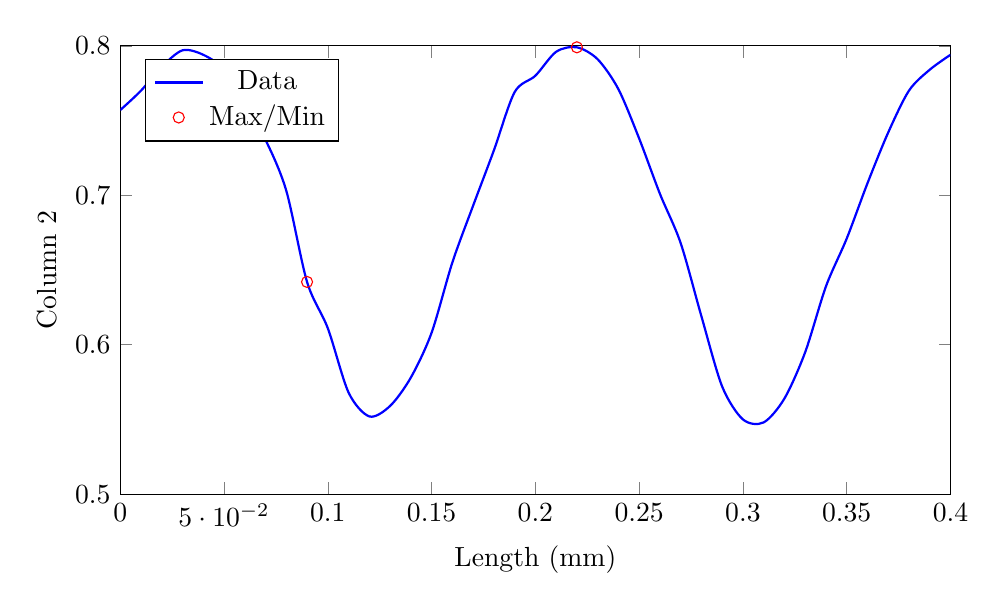
\begin{tikzpicture}
        \begin{axis}[
        width=\linewidth,
        height=0.6\linewidth,
        xmin=0, xmax=0.40,
        ymin=0.5, ymax=0.8,
        xlabel=Length (mm),
        ylabel=Column 2,
        legend pos=north west
        ]
        
        \addplot [smooth, thick, blue] table {
        0.00 0.757
        0.01 0.770
        0.02 0.786
        0.03 0.797
        0.04 0.794
        0.05 0.784
        0.06 0.760
        0.07 0.737
        0.08 0.703
        0.09 0.642
        0.10 0.611
        0.11 0.568
        0.12 0.552
        0.13 0.559
        0.14 0.578
        0.15 0.608
        0.16 0.655
        0.17 0.693
        0.18 0.730
        0.19 0.769
        0.20 0.780
        0.21 0.796
        0.22 0.799
        0.23 0.791
        0.24 0.771
        0.25 0.738
        0.26 0.701
        0.27 0.668
        0.28 0.619
        0.29 0.572
        0.30 0.550
        0.31 0.548
        0.32 0.564
        0.33 0.595
        0.34 0.639
        0.35 0.671
        0.36 0.708
        0.37 0.742
        0.38 0.770
        0.39 0.784
        0.40 0.794
        };
        
        \addplot [only marks, mark=o, red] coordinates {
        (0.22,0.799) % maximum point
        (0.09,0.642) % minimum point
        };
        
        \legend{Data,Max/Min}
        \end{axis}
        \end{tikzpicture}
    \end{figure}
    \end{landscape}


    \section{Matched Load}
    \begin{multicols}{2}
    \begin{table}[H]
        \centering
        \begin{tabular}{cc}
        \hline
        Length(mm) & Column 2 \\
        \hline
        0.00 & 0.752 \\
        0.01 & 0.750 \\
        0.02 & 0.742 \\
        0.03 & 0.735 \\
        0.04 & 0.721 \\
        0.05 & 0.692 \\
        0.06 & 0.674 \\
        0.07 & 0.647 \\
        0.08 & 0.629 \\
        0.09 & 0.610 \\
        0.10 & 0.598 \\
        0.11 & 0.598 \\
        0.12 & 0.613 \\
        0.13 & 0.614 \\
        0.14 & 0.634 \\
        0.15 & 0.655 \\
        0.16 & 0.673 \\
        0.17 & 0.698 \\
        0.18 & 0.724 \\
        0.19 & 0.743 \\
        0.20 & 0.751 \\
        0.21 & 0.742 \\
        0.22 & 0.730 \\
        0.23 & 0.715 \\
        0.24 & 0.685 \\
        0.25 & 0.666 \\
        0.26 & 0.640 \\
        0.27 & 0.625 \\
        0.28 & 0.606 \\
        0.29 & 0.601 \\
        0.30 & 0.601 \\
        0.31 & 0.607 \\
        0.32 & 0.623 \\
        0.33 & 0.642 \\
        0.34 & 0.668 \\
        0.35 & 0.697 \\
        0.36 & 0.718 \\
        0.37 & 0.734 \\
        0.38 & 0.744 \\
        0.39 & 0.744 \\
        0.40 & 0.738 \\
        \hline
        \end{tabular}
        \caption{Termination load}
    \end{table}
    \begin{table}[H]
        \begin{tabular}{|l|l|}
            \hline
            First Minimum value & \\ \hline
            First Maximum value & \\ \hline
            SWR value & \\ \hline
            Power reflected & \\ \hline
            
        \end{tabular}
    \end{table}
    \end{multicols}
    \begin{landscape}
    \begin{figure}[H] %ml
        \centering
        \textbf{Plot for Matched load with termination load}
        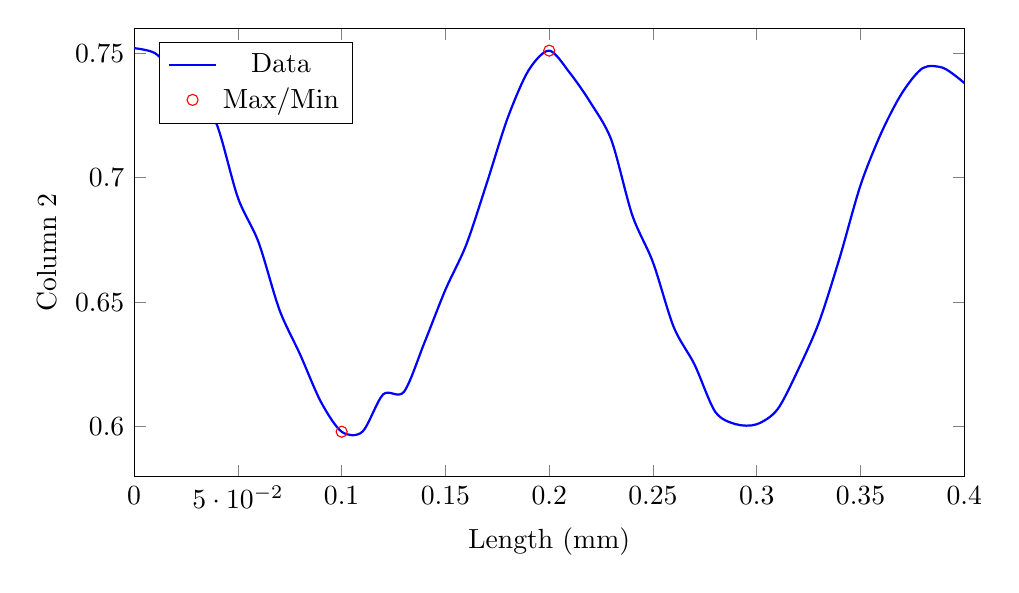
\begin{tikzpicture}
        \begin{axis}[
          width=\linewidth,
          height=0.6\linewidth,
          xmin=0, xmax=0.40,
          ymin=0.58, ymax=0.76,
          xlabel=Length (mm),
          ylabel=Column 2,
          legend pos=north west
        ]
        
        \addplot [smooth, thick, blue] table {
        0.00 0.752
        0.01 0.750
        0.02 0.742
        0.03 0.735
        0.04 0.721
        0.05 0.692
        0.06 0.674
        0.07 0.647
        0.08 0.629
        0.09 0.610
        0.10 0.598
        0.11 0.598
        0.12 0.613
        0.13 0.614
        0.14 0.634
        0.15 0.655
        0.16 0.673
        0.17 0.698
        0.18 0.724
        0.19 0.743
        0.20 0.751
        0.21 0.742
        0.22 0.730
        0.23 0.715
        0.24 0.685
        0.25 0.666
        0.26 0.640
        0.27 0.625
        0.28 0.606
        0.29 0.601
        0.30 0.601
        0.31 0.607
        0.32 0.623
        0.33 0.642
        0.34 0.668
        0.35 0.697
        0.36 0.718
        0.37 0.734
        0.38 0.744
        0.39 0.744
        0.40 0.738
        };
        
        \addplot [only marks, mark=o, red] coordinates {
        (0.20,0.751) % maximum point
        (0.10,0.598) % minimum point
        };
        
        \legend{Data,Max/Min}
        \end{axis}
        \end{tikzpicture}
    \end{figure}
    \end{landscape}


    \chapter{Explanation and Conclusion}


\end{document}